\documentclass{article}
\usepackage{amsmath}
\usepackage{amssymb}
\usepackage{graphicx}
\usepackage{hyperref}
\usepackage[version=4]{mhchem}


\begin{document}
In figure shown, \(A B C\) is a triangle with squares \(A B E F\) and \(A C G H\) drawn on sides \(A B\) and \(A C\), respectively. \(A D\) is the altitude of triangle \(A B C\). Prove that the extension of \(D A\) bisects \(F H\).

Proof:
Draw \(F P \perp D A\) at \(P, H Q \perp B C\) at \(Q\).\\
\centering
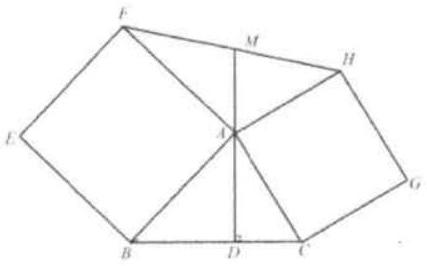
\includegraphics[width=\textwidth]{images/084.jpg}

Since \(\angle F A P+\angle B A D=90^{\circ}\), and \(\angle F A P+\angle A F P=90^{\circ}, \angle B A D=\angle A F P\).\\
We also know that \(H A F=A B, \angle A P F=\angle A D B=90^{\circ}\).\\
Thus Rt \(\triangle A P F \cong \mathrm{Rt} \triangle B D A\).\\
Similarly, we can show that Rt \(\triangle A H Q \cong\) Rt \(\triangle C A D\).\\
\centering
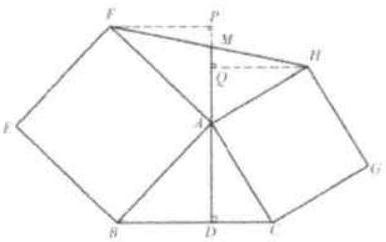
\includegraphics[width=\textwidth]{images/084(2).jpg}

So we have \(F P=A D=H Q\).\\
We also know that \(\angle F P M=\angle H Q M=90^{\circ}, \angle M F P=\angle M H Q\). Therefore \(\triangle F P M \cong\) \(\triangle H M Q\) and \(F M=M H\).


\end{document}
